\documentclass[conference]{IEEEtran}
% \IEEEoverridecommandlockouts
% The preceding line is only needed to identify funding in the first footnote. If that is unneeded, please comment it out.
\usepackage{cite}
\usepackage{amsmath,amssymb,amsfonts}
\usepackage{algorithmic}
\usepackage{graphicx}
\usepackage{textcomp}
\usepackage{xcolor}
\usepackage{xspace}
\usepackage[hidelinks]{hyperref}
\usepackage[a4paper, total={184mm,239mm}]{geometry}

\def\BibTeX{{\rm B\kern-.05em{\sc i\kern-.025em b}\kern-.08em
    T\kern-.1667em\lower.7ex\hbox{E}\kern-.125emX}}

%%%%%%%%%%%%%%%%%%%%%%%%%%%%%%%%%%%%%%%%%%%%%%%%%%%%%%%%%%%%%%%%%%%%%%%%%%%%%%%%%%%%%%
%     __________  ____  ____     _   ______  _________________
%    /_  __/ __ \/ __ \/ __ \   / | / / __ \/_  __/ ____/ ___/
%     / / / / / / / / / / / /  /  |/ / / / / / / / __/  \__ \
%    / / / /_/ / /_/ / /_/ /  / /|  / /_/ / / / / /___ ___/ /
%   /_/  \____/_____/\____/  /_/ |_/\____/ /_/ /_____//____/
%
% Thanks Patrick-san for the snippet
\usepackage{ifthen}
\newboolean{EnableTodoNotes}
\setboolean{EnableTodoNotes}{true}  % <<< set this to "false" to disable todos
\ifthenelse{\boolean{EnableTodoNotes}}{%
  \usepackage[colorinlistoftodos,prependcaption,obeyFinal,textsize=footnotesize]{todonotes}
  \paperwidth=\dimexpr \paperwidth + 6cm\relax
  \oddsidemargin=\dimexpr\oddsidemargin + 3cm\relax
  \evensidemargin=\dimexpr\evensidemargin + 3cm\relax
  \marginparwidth=\dimexpr \marginparwidth + 3cm\relax
}{%
  \usepackage[colorinlistoftodos,prependcaption,obeyFinal,disable]{todonotes}
}
\newcommand{\cf}[1]{\todo[color=pink!40]{\textbf{CF}: #1}}
\newcommand{\fls}[1]{\todo[color=cyan!40]{\textbf{FS}: #1}}


\begin{document}

\newcommand{\para}[1]{\vspace*{0.3\baselineskip}\noindent\textbf{#1.}}

\newcommand{\Pic}{Platform timing contract\xspace}
\newcommand{\pic}{platform timing contract\xspace}
\newcommand{\Pics}{Platform timing contracts\xspace}
\newcommand{\pics}{platform timing contracts\xspace}
\newcommand{\pici}{platform timing contract instrumentation\xspace}
\newcommand{\Pici}{Platform timing contract instrumentation\xspace}
\newcommand{\PICI}{PTCI\xspace}
\newcommand{\PICIs}{PTCIs\xspace}
\newcommand{\ucfi}{$\mu$CFI\xspace}

\title{Platform Timing Contracts: A Lightweight Instrumentation for Capturing SoC Timing Channels}

% \author{\IEEEauthorblockN{1\textsuperscript{st} Given Name Surname}
% \IEEEauthorblockA{\textit{dept. name of organization (of Aff.)} \\
% \textit{name of organization (of Aff.)}\\
% City, Country \\
% email address or ORCID}
% \and
% \IEEEauthorblockN{2\textsuperscript{nd} Given Name Surname}
% \IEEEauthorblockA{\textit{dept. name of organization (of Aff.)} \\
% \textit{name of organization (of Aff.)}\\
% City, Country \\
% email address or ORCID}
% \and
% \IEEEauthorblockN{3\textsuperscript{rd} Given Name Surname}
% \IEEEauthorblockA{\textit{dept. name of organization (of Aff.)} \\
% \textit{name of organization (of Aff.)}\\
% City, Country \\
% email address or ORCID}
% \and
% \IEEEauthorblockN{4\textsuperscript{th} Given Name Surname}
% \IEEEauthorblockA{\textit{dept. name of organization (of Aff.)} \\
% \textit{name of organization (of Aff.)}\\
% City, Country \\
% email address or ORCID}
% \and
% \IEEEauthorblockN{5\textsuperscript{th} Given Name Surname}
% \IEEEauthorblockA{\textit{dept. name of organization (of Aff.)} \\
% \textit{name of organization (of Aff.)}\\
% City, Country \\
% email address or ORCID}
% \and
% \IEEEauthorblockN{6\textsuperscript{th} Given Name Surname}
% \IEEEauthorblockA{\textit{dept. name of organization (of Aff.)} \\
% \textit{name of organization (of Aff.)}\\
% City, Country \\
% email address or ORCID}
% }

\maketitle

\begin{abstract}
Variations in the time a computer requires to perform computations can leak confidential information.
Constant-time programming techniques defend against such timing attacks, but make assumptions on the behavior of the underlying hardware.
As a response, previous work has introduced several techniques for verifying CPU compliance with hardware-software contracts.
%
However, selecting which hardware-software contract to verify is non-trivial and requires careful consideration of the system's architecture and the specific timing attacks it may face.
If a CPU is integrated into a platform with more timing channels than expected, CPU verification alone may be insufficient to guarantee security.
In this paper, we address the integration of a verified constant-time CPU into a larger system.
We make three contributions: (1) we define \pics as a formal way to capture an upper bound of the platform-induced timing channels, (2) we design a low-overhead synthetizable instrumentation that materializes these contracts and is compatible with all existing CPU verification methods, and (3) we demonstrate that existing CPU verification techniques along fail under integration, whereas \pics enable stronger, system-wide security guarantees against timing attacks.

% We introduce platform timing contracts, a novel abstraction that specifies an upper bound on timing channels introduced by platform integration.
% We introduce a lightweight instrumentation that allows for the dynamic monitoring of platform-induced timing channels and that is inherently compatible with all CPU constant-time verification techniques.
% Based on this instrumentation, we show that several techniques, while effective in isolation, fail to provide security guarantees when the CPU is integrated into a larger system.

\end{abstract}

% \begin{IEEEkeywords}
% component, formatting, style, styling, insert
% \end{IEEEkeywords}

%-------------------------------------------------------------------------------
\section{Introduction} \label{sec:introduction}
%-------------------------------------------------------------------------------
% !TeX root = ../main.tex
% !TeX spellcheck = en_US

\textcolor{red}{Should not only be about uarch. Should also be about archi leakage also?}
Microarchitectural attacks are software-driven techniques that exploit behaviors below the ISA to encode and reveal secrets through measurable side effects, most commonly execution time.
By carefully choreographing benign-looking instruction sequences, an attacker steers microarchitectural state, such as caches, TLBs, execution ports, branch predictors, DRAM buffers, to make secret-dependent effects externally observable.
Two broad families have emerged: transient/speculative-execution attacks~\cite{kocher2019spectre,lipp2018meltdown,armsecure,bhattacharyya2019smotherspectre,van2018foreshadow,canella2019fallout,horn2018speculative,maisuradze2018ret2spec,schwarz2019zombieload,schwarz2019netspectre,stecklina2018lazyfp,van2019ridl,ragab2021crosstalk,van2020lvi,van2021cacheout,ragab2021rage,wikner2022retbleed,trujillo2023inception,wikner2023phantom,wikner2024breaking,wikner2025bpi}, which leave secret-dependent footprints during mis-speculated execution, and contention-driven channels on shared resources~\cite{bernstein2005cache,bonneau2006cache,Liu2015LLC,YaromFalkner2014FlushReload,Gras2018TLBleed,Aldaya2019PortSmash,Yarom2016CacheBleed,Moghimi2018MemJam,Gruss2016PrefetchSCA,Pessl2016DRAMA}, which measure or induce interference to encode information.
These attacks pose a durable, cross-generation threat to modern processors, in particular because they can be mounted entirely in software, without special privileges or hardware access.
Mitigation is notoriously difficult once silicon has shipped: the leakage channels are entwined with performance-critical design choices.
Software or microcode defenses are often partial~\cite{ridlad} or impose significant overheads.

To inform software developers about the potential side effects of their code on a given contract-compliant CPU, recent work has introduced hardware-software contracts~\cite{guarnieri2021hardware,oleksenko2022revizor}.
As a result, several techniques have been proposed to formally verify that a CPU implementation complies with such contracts~\cite{dinesh2024conjunct,dinesh2025h,ceesay2024mucfi,wang2023specification,tan2025contractshadowlogic,hsiao2024rtl2mmupath} to prevent confidentiality breaches before chip fabrication.

\para{Platform timing channels}
CPUs are often verified in isolation~\cite{dinesh2024conjunct,dinesh2025h,ceesay2024mucfi,wang2023specification,tan2025contractshadowlogic,hsiao2024rtl2mmupath} before integration into a larger system, often for scalability reasons.
Yet hardware-software contracts make assumptions on the system into which a CPU will be integrated.
For example, the constant-time contract observer mode~\cite{guarnieri2021hardware} exposes the program counter of every executed instruction, and the addresses of all memory operations.
This observation mode accounts for the timing effects of caches and other elements of the memory hierarchy~\cite{guarnieri2021hardware,oleksenko2022revizor}.
Other contract observation modes exist, for example the architectural observer, which additionally discloses values exchanged with memory.
These aspects of hardware-contracts are proper to the platform (i.e., the broader SoC) into which the CPU will be integrated, yet many verification techniques do not account for them or provide this flexibility.

\para{Platform timing contracts}
Platform timing contracts extend the idea of hardware-software contracts to encompass the broader system context in which a CPU operates.
They aim to capture the timing behavior of the entire platform, including interactions with other components such as memory controllers, I/O devices, and interconnects.
By considering these interactions, platform timing contracts can provide a more comprehensive understanding of potential timing channels and their implications for security.
To verify the compliance of a CPU integrated into a specific platform using existing techniques that verify a CPU in isolation, we introduce an automatic instrumentation that captures the relevant platform-specific timing information while retaining compatibility with all existing hardware-software contract verification techniques.

We establish the platform timing contracts for \textcolor{red}{3} different platforms.
We apply the instrumentation corresponding to each platform to the \textcolor{red}{4} RISC-V CPUs \textcolor{red}{TODO List them}.
Not only does the verification time increase by not more than ~\textcolor{red}{5}\%, but we demonstrate the existence of platform-specific timing channels on typical platforms, that would otherwise be missed.

In summary, our contributions in this paper are:
\begin{itemize}
    \item We introduce \pics.
    \item We implement an open-source lightweight CPU instrumentation that accounts for all platform-induced timing side-channels.
    \item We apply instrumentations corresponding to various platforms to the 4 RISC-V CPUs to capture platform-specific timing information and show that these platforms can introduce unique timing channels that may not be present in isolated CPU verification and that would be missed by some existing verification techniques.
\end{itemize}

\vspace*{0.5em}
All our experiments can be found at: \url{https://placeholder/} 

% % TODO Say the importance of platform side channels.

% % Microarchitectural attacks exploit subtle CPU features to encode and leak sensitive information through program execution time. Because they can be mounted entirely from software, they pose a significant long-term threat to modern CPUs.
% % They may exploit speculative execution~\cite{kocher2019spectre,lipp2018meltdown,armsecure,bhattacharyya2019smotherspectre,van2018foreshadow,canella2019fallout,horn2018speculative,maisuradze2018ret2spec,schwarz2019zombieload,schwarz2019netspectre,stecklina2018lazyfp,van2019ridl,ragab2021crosstalk,van2020lvi,van2021cacheout,ragab2021rage} or resource contention~\cite{bernstein2005cache,bonneau2006cache,Liu2015LLC,YaromFalkner2014FlushReload,Gras2018TLBleed,Aldaya2019PortSmash,Yarom2016CacheBleed,Moghimi2018MemJam,Gruss2016PrefetchSCA,Pessl2016DRAMA}.
% % They are notoriously difficult to mitigate once hardware has been fabricated.

% Traditionally, these vulnerabilities were looked for manually~\cite{dessouky2019hardfails} or using dynamic techniques that are as good as their test cases~\cite{weber2021osiris,ghaniyoun2021introspectre,de2025phantom,hur2022specdoctor,rostami2024lost,borkar2024whisperfuzz,oleksenko2022revizor}.
% Recently, advances in speculation contracts~\cite{guarnieri2021hardware} and relational reasoning~\cite{oleksenko2022revizor} have formalized the problem of proving the absence of timing channels in CPUs as a \emph{non-interference} property.
% Intuitively, a CPU complies with such a non-interference property if the program's secret data does not affect the CPU's observable behavior, if the program complies with some understanding of constant-time property.
% For example, the program shall not use the secret data as the input to a branch if adversaries can observe branch decisions.
% Such program constraints can be understood as variants of constant-time programming.

% Several dedicated verification schemes have been proposed in the last few years.
% They formally prove the absence of an information leakage from secret data to observable channels such as timing, generally based on one of two properties named \emph{Safe Instruction Set} (SIS) and the stronger \emph{Speculative Non-Interference} (SNI).
% Despite being different properties, both guarantee that secret information computed in a CPU cannot be inferred from the system's observable behavior if the software is written in a constant-time manner.
% However, all the so-far-proposed techniques for formally proving constant-time properties in CPUs make explicit or implicit assumptions on the system into which the CPU will be integrated, and on the implementation of the CPU under verification or on the systems that integrate it.
% \fls{We might also say something about the threat model / about SoCs that have external IPs.}

% \para{\Pics}
% Some information flows that can reveal secrets might exit the CPU to reenter it and affect its timing, and might escape the scope of verification techniques through these reentrant paths. 
% The existence and nature of such reentrant information flows depend on the system into which the CPU is integrated.
% Yet, no existing constant-time verification technique addresses this issue explicitly.
% Some techniques ignore reentrant information flows altogether~\cite{ceesay2024mucfi,dinesh2024conjunct,dinesh2024conjunct}.
% We will see that this can lead to missing vulnerabilities that would be otherwise detectable when the CPU is integrated into a larger system.
% Others techniques may assume the existence of address-dependent timing channels~\cite{wang2023specification,tan2025contractshadowlogic}, due for example to caches present in the system.
% To address this issue, we introduce \pics, a simple specification of the reentrant information flows that exit and reenter the CPU.
% Based on this specification, we introduce an automatic lightweight instrumentation that augments a CPU with a synthesizable summary of all the potential reentrant information flows from the platform that integrates the CPU.

% \para{Assumptions in constant-time verification}
% We note that unsoundness is not only due to reentrant information flows, but also due to assumptions made by the verification techniques.
% We analyze the assumptions that underpin the automatic state-of-the-art non-interference property verification techniques, once the reentrant flow challenge is addressed.
% We find that these assumptions can be categorized into three classes.
% (a) The \emph{Correctness Assumption}: a CPU shall be exempt from functional bugs.
% % In this paper, we find that a well-defined class of functional correctness bugs, which are common even in widely-adopted CPUs~\cite{solt2022rememberr}, can cause unsoundness under this assumption.
% In this paper, we demonstrate that indeed functional correctness bugs can cause unsoundness for techniques that formulate this assumption.
% Further, we identify that only a well-defined class of functional correctness bugs can lead to such unsoundness.
% (b) The \emph{Architectural Flow Matching Assumption}: information flows on architectural paths shall coincide with architectural transactions.
% In this paper, we show that microarchitectural transactions that are not architectural, such as microarchitecturally reading architectural values during transient execution, can cause unsoundness for techniques that formulate this assumption.
% (c) The \emph{Input Constraint Assumption}: some input data words shall be constrained to a restricted set of potential values interpreted as safe instruction encodings.
% In this paper, we show that an increase in the diversity of input words, such as the cohabitation of data and instructions on a memory bus, is typical when the CPU is integrated into a larger system, and can cause unsoundness for techniques that formulate this assumption.
% Taken individually, each of these three assumptions is generally violated in typical CPU implementations.

% \para{Inconstant}
% Intuitively, each verification technique has its own strengths and weaknesses.
% For example, the contract shadow logic technique~\cite{tan2025contractshadowlogic} relies on the correctness assumption, while \ucfi has been demonstrated to have practical functional correctness bug detection capabilities~\cite{ceesay2024mucfi}, hence one might expect complementarity between these two techniques.
% Unfortunately, we show that not only does each verification technique have its own assumption-related blind spots, but even if we combine all automatic state-of-the-art verification techniques~\cite{dinesh2024conjunct,dinesh2025h,ceesay2024mucfi,wang2023specification,tan2025contractshadowlogic}, common blind spots remain that cannot be detected, which fundamentally undermines the typical comprehensiveness expectations that verification engineers have when using formal techniques.
% % To demonstrate the existence of common blind spots, we construct \cpuname, a RISC-V CPU implementation based on the 2-stage Sodor implementation~\cite{sodor}.
% % \ourname contains an information leakage vulnerability that we craft by leveraging our classification and analysis of the assumptions made by the state-of-the-art verification techniques, and we demonstrate the existence of a timing side-channel in \ourname that is undetectable by all the existing automatic constant-time verification techniques combined.
% We formulate a set of guidelines to help researchers and practitioners reason about constant-time verification techniques.
% % \textbf{(I'm not yet sure what the guidelines will be but it would be a nice-to-have)}
% % }

% \ourname is available at \url{https://comsec.ethz.ch/hybridift/}


%-------------------------------------------------------------------------------
\section{Background} \label{sec:background}
%-------------------------------------------------------------------------------
In this section, we provide background on SoC platforms, timing side-channels and non-interference properties.

\subsection{SoC platforms}

\begin{figure}[t]
    \begin{center}
    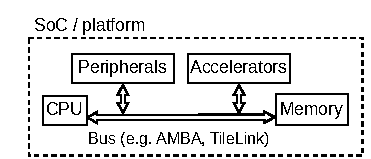
\includegraphics[width=0.8\columnwidth]{figures/exampleplatform/exampleplatform.pdf}
    \end{center}
    \vspace*{-1em}
    \caption{\label{fig:exampleplatform}
        Example SoC platform architecture.
    }
    \vspace*{-1em}
\end{figure}

In this paper, we use the words SoC, system and platform interchangeably to refer to the integrated circuit that integrates various components, including CPUs, memory, and peripherals, as illustrated in Fig.~\ref{fig:exampleplatform}.
The communication between these components is typically managed through standardized bus protocols, such as AMBA~\cite{arm_amba} or TileLink~\cite{tilelink_spec}.
The bounds of components are not always clear-cut.
For example, Fig.~\ref{fig:verifscopecache} shows that caches can be considered part of the CPU or of the rest of the platform.
For a hardware component, we refer to its \emph{input signals} as the inbound wires, and its \emph{inputs} as the values carried by those wires, and similarly for outputs.

\subsection{Timing side-channels}

Multiple hardware optimizations, such as caches and branch predictors, learn and exploit patterns in program execution to improve performance.
In particular, the execution time of later instructions may depend on the outcome of earlier instructions.
For example, accessing a cache line might be faster if the line has been brought into the cache recently by a prior memory access to a nearby location.
% Timing side channels can result from such optimizations when the timing of a program's execution depends on secret data.
Constant-time programming techniques, such as not using secret data as array indices or loop conditions, aim to ensure that secrets do not influence the execution time of a program through such channels~\cite{OsvikShamirTromer2006CacheAES,AlmeidaEtAl2016CTVerif}.

\subsection{Information Flow Tracking}
\label{subsec:ift}

\begin{figure}[t]
    \begin{center}
    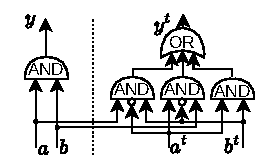
\includegraphics[width=0.5\columnwidth]{figures/glift/glift.pdf}
    \end{center}
    \vspace*{-1em}
    \caption{\label{fig:glift} Taint tracking at gate level~\cite{tiwari2009complete}. Left: original circuit. Right: Added instrumentation for taint tracking. The original input signals are $a$ and $b$. The taint bits corresponding to $a$ and $b$ are respectively $a^t$ and $b^t$. The output taint bit $y^t$ indicates whether the output is tainted, i.e., influenced by the tainted inputs.}
    \vspace*{-1em}
\end{figure}

\begin{figure}[t]
    \begin{center}
    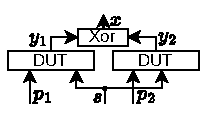
\includegraphics[width=0.5\columnwidth]{figures/miter/miter.pdf}
    \end{center}
    \vspace*{-2em}
    \caption{\label{fig:miter} Miter circuit. The two instances of the same DUT are supplied with the same public data $p$ and unconstrained $s_1$ and $s_2$ secret data. The output bit $y$ (i.e., instantiated for the instances in the miter as $y_1$ and $y_2$) reveals secret data if $x=1$ is satisfiable.}
    % \vspace*{-1em}
\end{figure}

Hardware information flows capture properties such as confidentiality and integrity~\cite{hu2021hardware}.
They are typically tracked using one of two techniques.
The first technique is called dynamic information flow tracking (DIFT).
It captures information flows by augmenting the hardware design under test (DUT) with a synthesizable instrumentation that computes the propagation of taint bits~\cite{tiwari2009complete,ardeshiricham2017register,solt2022cellift,solt2024hybridift,ceesay2024mucfi} as shown in Fig.~\ref{fig:glift}.
The second technique is called a miter circuit.
It captures information flows by comparing the outputs of two copies of the DUT, where all inputs except the sources are unconstrained, while all the others are equal as illustrated in Fig.~\ref{fig:miter}.

\subsection{Hardware-software contracts}
\label{subsec:hw-sw-contracts}

\para{Contract definition}
Hardware-software contracts~\cite{guarnieri2021hardware} split confidentiality responsibilities between the CPU and the software that it executes.
For an initial microarchitectural state, a given program $P$, and the contents of memory containing public information $M_p$ and secret information $M_s$, the contract specifies an execution mode and an observation mode.
The \emph{execution mode} determines which instructions are executed (potentially transiently) and generate events.
The \emph{observation mode} determines which of those events are exposed to an observer (possibly transiently), such as the addresses or values involved in memory accesses.
Under such a contract, the CPU's behavior is summarized as a sequence of observable events known as a hardware trace~\cite{guarnieri2021hardware,oleksenko2022revizor}.

\para{Contract verification}
Multiple independent verification efforts have been conducted to ensure that hardware-software contracts are upheld during program execution, in particular regarding constant-time behavior~\cite{dinesh2024conjunct,ceesay2024mucfi,guarnieri2021hardware,tan2025contractshadowlogic,dinesh2025h,hsiao2024rtl2mmupath,wang2023specification}.
Most techniques consider a fixed contract~\cite{dinesh2024conjunct,ceesay2024mucfi,tan2025contractshadowlogic,dinesh2025h}, while some others leverage custom, non-trivial technique-specific insights to verify a wider variety of contracts~\cite{hsiao2024rtl2mmupath,wang2023specification} using the same technique.

\para{Discussion}
These techniques make assumptions about the platform in which the CPU is integrated, yet there exists no language for formally expressing and verifying them.


%-------------------------------------------------------------------------------
\section{\textcolor{red}{Reentrancy}} \label{sec:reentrant}
%-------------------------------------------------------------------------------
\subsection{Motivational example}

In this section, we first provide a motivational example showing that the integration of a CPU into a platform can introduce new timing channels that were not present in isolation.
We then discuss and formalize reentrant information flows.
Finally, we introduce platform integration contracts to capture these reentrant flows.

\begin{figure}[t]
    \begin{center}
    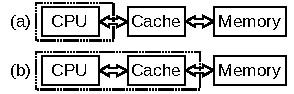
\includegraphics[width=0.6\columnwidth]{figures/verifscopecache/verifscopecache.pdf}
    \end{center}
    \vspace*{-1em}
    \caption{\label{fig:verifscopecache}
        Example verification scopes, represented as dotted boxes. (a: cache excluded) the cache is considered part of the platform. (b: cache included) the cache is considered part of the CPU.
    }
    \vspace*{-1em}
\end{figure}


\para{Methodology (cache excluded)}
Figure~\ref{fig:verifscopecache} (a) illustrates a small system in which a CPU is integrated in a platform that includes a cache and memory.
We instantiate this system, using the Kronos CPU as a case study, and a direct-mapped cache.
We use the state-of-the-art VeloCT~\cite{dinesh2025h} tool to perform constant-time verification of the CPU, which is delimited by the dotted box.
This tool verifies if only instructions of a given "safe instruction set" are executed, then the CPU runtime is independent of their operands.
We consider memory instructions as part of the safe instruction set that should execute in constant-time, in addition to arithmetic RISC-V instructions such as \texttt{add}, \texttt{sub}, \texttt{xor}, etc.

\para{Results (cache excluded)}
The Kronos verification with VeloCT, which indicates that in isolation, the CPU is constant-time secure.
In particular, this result suggests that the timing of any program made of arithmetic and memory instructions does not depend on the data that is processed, even if this data is used as memory addresses.

\para{Methodology (cache included)}
Figure~\ref{fig:verifscopecache} (b) illustrates a scenario similar to Figure~\ref{fig:verifscopecache} (a), but with the cache included in the verification scope, i.e., considered part of the CPU under verification.
Except for this point, we use the same methodology as in the previous cache excluded case.

\para{Results (cache included)}
The Kronos verification with VeloCT, which indicates that this time, the CPU is not constant-time secure.
In particular, this result implies that the program execution timing can depend on secret information used as addresses of memory instructions.

\para{Take-aways}
These results underline that while constant-time verification techniques typically operate at the level of a CPU in isolation (the platform's RTL might not yet be finalized at the CPU verification time), they may not account for all the potential interactions with other components in the system, such as caches or memory.
Therefore, the integration of the CPU into a larger system can introduce new timing channels that were not present in isolation and that are not discovered by existing constant-time verification techniques.

\subsection{Reentrant flows}

We now describe and formalize reentrant information flows, which are at the core of the timing channels that can be introduced by platform integration.

\para{Netlist graphs}
We describe a digital hardware system (e.g., the one illustrated in Figure~\ref{fig:verifscopecache}), as a netlist $G = (V, E)$, where $V$ is the set of vertices representing logic gates such as AND, OR, NOT, flip-flops, adders, and $E$ is the set of directed wires between these vertices.
We denote the subgraph of $G$ that corresponds to the CPU that is integrated in this system as $G_C = (V_C, E_C)$, where $V_C \subseteq V$ and $E_C \subseteq E$.
In particular, for all edges $(u, v) \in E_C$, both $u$ and $v$ are vertices in $V_C$.
We denote the complementary subgraph as $G_{P} = (V_{P}, E_{P})$, where $V_{P} = V \setminus V_C$ and $E_{P} = E \setminus E_C$, corresponding to the platform except the CPU that it integrates.

\para{Constant-time programs \& secret data}
For a given constant-time verification technique, let us denote by $\mathcal{P}$ the set of constant-time programs that are considered for verification.
The elements of the set $\mathcal{P}$ are triples $\tau = (P, M_p, M_s)$, where $P$ is a constant-time program, $M_p$ is the set of public memory valuations, and $M_s$ is the set of secret values that the program may depend on.
Specifically, this set $\mathcal{P}$ depends on the specific constant-time verification technique being used.
For example, for ConjunCT~\cite{dinesh2024conjunct} and VeloCT~\cite{dinesh2025h}, a triple ($P$, $M_p$, $M_s$) is considered constant-time (i.e., part of $\mathcal{P}$) if it contains no so-called "unsafe" instructions, i.e., instructions that can create an operand-dependent timing channel.
For Tan et al.~\cite{tan2025contractshadowlogic}, a triple ($P$, $M_p$, $M_s$) is considered constant-time (i.e., part of $\mathcal{P}$) if it ensures that the program's control flow and all memory accesses are independent of secret data.
The conditions for a program to be constant-time with respect to ConjunCT's and VeloCT's definition are stricter than those of Tan et al.~\cite{tan2025contractshadowlogic}, as the latter generally forbid branches, for instance.
Inclusively more restrictive constraints imply an inclusively smaller set $\mathcal{P}$ of constant-time programs.

\para{Secret propagation}
Constant-time verification techniques generally proceed by analyzing whether the valuation of a state element that captures timing differences can be influenced by secret information.
For example, Tan et al.~\cite{tan2025contractshadowlogic}, LeaVe~\cite{wang2023specification}, ConjunCT~\cite{dinesh2024conjunct} and VeloCT~\cite{dinesh2025h} monitor whether secret information can influence the commit signal, while \ucfi~\cite{ceesay2024mucfi} monitors whether secret information can influence a microarchitectural program counter structure.

We define the \emph{valuation sequence} $\nu$ of a vertex.
For a vertex $v \in V$ and a triple $\tau = (P, M_p, M_s)$, the valuation sequence $\nu_\tau(v)$ is the clock-accurate infinite sequence of valuations that the vertex takes during the execution of a program $P$ with respect to the memory valuations $M_p$ and $M_s$, starting from the CPU's and platform's reset state, assumed deterministic.
Note that we assume determinism for simplicity without loss of generality; to account for non-determinism, we could consider a set $\nu_\tau^{\text{non-det}}(v)$ of all possible valuation sequences instead of a single sequence $\nu_\tau(v)$, without change in the following reasoning.

We denote by $V^s$ the set of vertices in $V$ whose valuation sequence can be influenced by secret information when the system executes a program written in constant-time with respect to the secret data.
An element $v \in V$ belongs to $V^s$ if and only if there exist two triples $\tau = (P, M_p, M_s)$ and $\tau' = (P, M_p, M_s')$ that only differ in $M_s'$, and such that $\tau \in \mathcal{P}$ and $\tau' \in \mathcal{P}$ but $\nu_\tau(v) \neq \nu_{\tau'}(v)$.
We say that a vertex $v \in V$ is \emph{secret-dependent} if it belongs to $V^s$.

For a secret-dependent vertex $v \in V^s$, we define the set $P^s_v$ of \emph{secret propagation paths} to be the paths in the graph $G$ that connect the source of secrets (that can take the value $M_s$ or $M_s'$) to $v$, where all the vertices in the path are secret-dependent.
In particular, $P^s_v$ is non-empty.
Indeed, if $v \in V^s$, then at least one predecessor $u \in V$ of $v$ must also be secret-dependent, which recursively constructs a path in $P^s_u$.

Let us consider a strict subgraph $G' = (V', E') \subsetneq G$ and a vertex $v \in V'^s$.
A path $p$ in $P^s_v$ is said to be \emph{reentrant} in $G'$ if it contains at least one vertex $u \in V \setminus V'$, i.e., a vertex that is outside of $G'$.
Note that this $u$ also belongs to $V^s\setminus V'$ because all nodes in $p$ are secret-dependent by definition of $P^s_v$.
If all paths in $P^s_v$ are reentrant in $G'$, then we say that the vertex $v$ is \emph{fully reentrant} in $G'$.

\para{Example}
Let us consider again the system Figure~\ref{fig:verifscopecache} (a) where $\mathcal{P}$ describes programs where secret data, which is for example initially stored in a well-specified general-purpose register, can be used as the address of a memory instruction.
Because the CPU itself does not contain caches or other components whose timing depends on memory addresses, for $v$ designating the commit signal (for LeaVe~\cite{wang2023specification}, Tan et al.~\cite{tan2025contractshadowlogic}, ConjunCT~\cite{dinesh2024conjunct} or VeloCT~\cite{dinesh2025h}), or a microarchitectural PC signal (\ucfi~\cite{ceesay2024mucfi}), $v$ is fully-reentrant in the CPU, if we consider $G$ being the whole platform, and $G'$ being the CPU.

\subsection{Contracts}

The key idea of our work is to define \emph{platform timing contracts} that capture the possible reentrant information flows in the CPU that are allowed by a given platform.
Since the interface between the output signals of a CPU and the rest of a SoC is usually much simpler than the hardware-software interface, these contracts are expected to be simpler than existing hardware-software contracts.

\para{Interface}
We base our analysis on the widely-studied RISC-V ISA.
The output signals of a RISC-V CPU are all through memory interfaces, which are made of data and control signals.
% \fls{TODO Maybe change all "CPU"'s with "CPU core"}
Data signals transport the data to be read or written to or from the memory.
Control signals transport the information about the memory transaction, such as the memory address, handshake signals, and depending on the memory bus protocol (e.g., AMBA AXI~\cite{arm_amba} or TileLink~\cite{tilelink_spec}), further control signals such as the type of transaction and the size of the data to be read or written.
Input signals of a RISC-V CPU can be more diverse, including memory input data and control signals, interrupt lines, and various other control signals such as clock gating signals.

\para{Platform timing contracts}
Platform timing contracts aim to ensure that state elements that capture timing differences (e.g., a commit signal or a microarchitectural program counter) \emph{are not fully reentrant} in the CPU.
To ensure this, a platform timing contract specifies an upper bound of the information flows between the output signals of the CPU and its input signals.
We express a platform timing contract as a list of rules, listed per CPU output signal.
% In Section~\ref{sec:instrumentation}, we introduce synthesizable constructs that create paths between secret sources and sinks, to ensure that the sets $P^s_v$ are not empty for these sinks, preventing these sinks from being fully-reentrant.
% \textcolor{red}{TODO Continuer ici.}


\para{Example contracts}
Fig.~\ref{fig:contract_equations} provides four example contracts for a RISC-V CPU with a Von Neumann architecture.
We model the memory interface as an outbound address bus (\texttt{addr}), an inbound and an outbound memory data port (respectively \texttt{rdata} and \texttt{wdata}), and a simple valid-ready handshake protocol (inbound \texttt{resp} and outbound \texttt{req}), similar to the \texttt{req} and \texttt{gnt} handshake signals in the Hardware Processing Engines (HWPE) 2.0 interface protocol~\cite{pulpHWPEMem}.
Fig.~\ref{fig:contract_equations}'s contract C1 defines a simple integration contract for a platform with ideal memory that responds with a constant timing (i.e., that is address-independent).
A change in the memory transaction control signals from the CPU can only change the returned value.
Only the request signal (\texttt{req}) can affect the existence, and hence the timing, of a memory response.
% Indeed, a change in the address of a read, for example, might read from a memory cell that contains a different value, and a change, for example in the timing of some request signal will affect the timing of the memory response, and hence the memory read data at some point in time.
The diamond $\lozenge$ underlines that the right-hand side of the implication can happen at any time and for any number of times after the left-hand side.
% \fls{Maybe I should explain more intuitions like why req and addr actually have exactly the same effect.}
Equation~\ref{dict:contract_cache_nointerrupt} adds timing dependence on the memory address, which is typical of structures like caches.
In this contract, \texttt{req} and \texttt{addr} have an identical clause. Indeed, a change in the address of a read, for example, can change a cache miss into a cache hit, changing the timing, and hence the value at some point in time, of the response, including the \texttt{gmt} control signal and the \texttt{rdata} data signals.
Equation~\ref{dict:contract_cache_interrupt} models data-dependent interrupts and timing, which might occur, for example, if some peripheral can be controlled through memory-mapped registers such as an interrupt controller~\cite{riscv_plic_spec_1_0_0}.

\para{Conditional refinements}
\fls{TODO ensure to reference section III.B.}
Equation~\ref{dict:contract_cache_interrupt} implies that writing tainted, i.e., secret, data to memory with a specific address that is not tainted might always trigger an interrupt or affect the timing of the memory response. In some settings, this might be true only for specific address ranges where peripherals are mapped, but parts of the memory address range can typically be used in a data-independent timing.
\fls{Be more concrete here.}
To refine this contract, we introduce address-dependent contracts as in Equation~\ref{dict:contract_cache_interrupt_addressdependent}, where the right-hand side of the implication depends on the memory address set \texttt{periph\_range}, which is a fixed set of addresses.
% Note that the contract could also be refined by making the interrupts dependent on the written data.
% For example, an interrupt might never be triggered, whatever the address, if the written data is zero, for the class of platforms of interest for the CPU integrator.
% In verification, such constraints can be expressed as data-independent timing assuming that the CPU does not write to memory addresses in \texttt{periph\_range} with tainted data.
For example, this can be achieved with RISC-V Physical Memory Protection (PMP) in a setting where the most privileged execution mode does not access secret data and protects the \texttt{periph\_range} address range from being accessed from lower privileges, in the philosophy of trusted execution environments~\cite{lee2019keystone,costan2016sanctum,arm2009trustzone,mcgillion2015opentee,schneider2022sok,bourgeat2018mi6,brasser2022tcx}.

% \fls{TODO Say that we will have a reference contract later for the end-to-end attack.}
% \fls{TODO Say the right-hand side can be anytime after, and for any number of time. Maybe write this as an LTL formula.}


\begin{figure}
    \begin{center}
    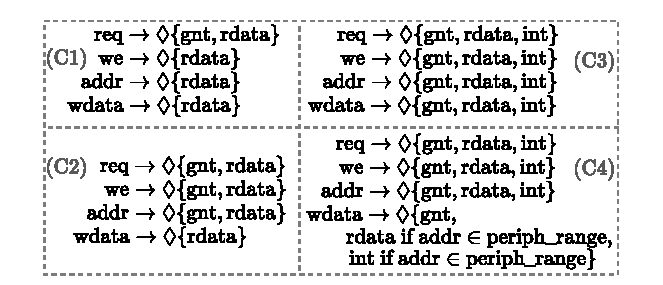
\includegraphics[width=\columnwidth]{figures/contract_equations/contract_equations.pdf}
    \end{center}
    \vspace{-1.8em}
    \caption{Example platform contracts.}
    \label{fig:contract_equations}
    \vspace*{-1.5em} 
\end{figure}

% \begin{equation}
% \label{dict:contract_nocache}
% \begin{array}{rcl}
% \text{req} & \rightarrow & \lozenge \{ \text{gnt}, \text{rdata}\} \\
% \text{we} & \rightarrow & \lozenge \{\text{rdata}\} \\
% \text{addr} & \rightarrow & \lozenge \{ \text{rdata}\} \\
% \text{wdata} & \rightarrow & \lozenge \{ \text{rdata} \} \\
% \end{array}
% \end{equation}

% \begin{equation}
% \label{dict:contract_cache_nointerrupt}
% \begin{array}{rcl}
% \text{req} & \rightarrow & \lozenge \{ \text{gnt}, \text{rdata}\} \\
% \text{we} & \rightarrow & \lozenge \{ \text{gnt}, \text{rdata}\} \\
% \text{addr} & \rightarrow & \lozenge \{ \text{gnt}, \text{rdata}\} \\
% \text{wdata} & \rightarrow & \lozenge \{ \text{rdata} \} \\
% \end{array}
% \end{equation}

% \begin{equation}
% \label{dict:contract_cache_interrupt}
% \begin{array}{rcl}
% \text{req} & \rightarrow & \lozenge \{ \text{gnt}, \text{rdata}, \text{interrupt}\} \\
% \text{we} & \rightarrow & \lozenge \{ \text{gnt}, \text{rdata}, \text{interrupt}\} \\
% \text{addr} & \rightarrow & \lozenge \{ \text{gnt}, \text{rdata}, \text{interrupt}\} \\
% \text{wdata} & \rightarrow & \lozenge \{ \text{gnt}, \text{rdata}, \text{interrupt} \} \\
% \end{array}
% \end{equation}

% \begin{equation}
% \label{dict:contract_cache_interrupt_addressdependent}
% \begin{array}{rcl}
% \text{req}  & \rightarrow & \lozenge \{ \text{gnt}, \text{rdata}, \text{interrupt}\} \\
% \text{we}  & \rightarrow & \lozenge \{ \text{gnt}, \text{rdata}, \text{interrupt}\} \\
% \text{addr} & \rightarrow & \lozenge \{ \text{gnt}, \text{rdata}, \text{interrupt}\} \\
% % \text{wdata} & \rightarrow & \lozenge \{ \text{rdata}, \text{interrupt} \} \\
% \text{wdata} & \rightarrow & \lozenge \{ \text{rdata}, \\
% & & \text{gnt if addr in periph\_range} \\
% & & \text{interrupt if addr in periph\_range} \} \\

% \end{array}
% \end{equation}

\para{Ordering of \pics}
Like for sinks, we can define a partial ordering of \pics.
We say that a contract A is (inclusively) stronger than a contract B if for every output of the CPU (i.e., the left-hand side of the arrow in the contract), the set of possible CPU inputs tainted by this output in contract A is a subset of the set of possible CPU inputs tainted by this output in contract B.
Said otherwise, contract A is stronger than contract B if it allows for fewer possible information flows.
For example, Equation~\ref{dict:contract_cache_interrupt_addressdependent} is stronger than Equation~\ref{dict:contract_cache_interrupt}, and Equation~\ref{dict:contract_cache_nointerrupt} is stronger than Equation~\ref{dict:contract_cache_interrupt}.
A CPU that is verified to have a constant-time behavior with respect to a stronger \pic is also verified with respect to a weaker \pic.

\begin{figure}
    \begin{center}
    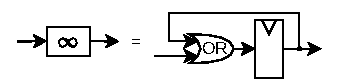
\includegraphics[width=.7\columnwidth]{figures/stickyone/stickyone.pdf}
    \end{center}
    \vspace*{-1em}
    \caption{Sticky-one operator. The sticky-one is reset to zero (not illustrated in the figure) and sticks to 1 once it is set.}
    \label{fig:stickyone}
    \vspace*{-.4em}
\end{figure}


\begin{figure}[t]
    \begin{center}
    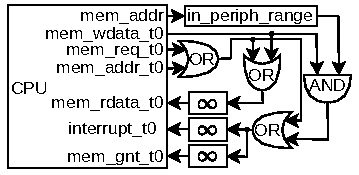
\includegraphics[width=.7\columnwidth]{figures/picinstrum_taints/picinstrum_taints.pdf}
    \end{center}
    \vspace*{-1em}
    \caption{\Pici for a design whose information flows are tracked with dynamic information flow tracking instrumentation. Signals that end with \texttt{t0} represent the taint signals~\cite{tiwari2009complete,solt2022cellift}.
    }
    \label{fig:pic_instrum_taints}
    \vspace*{-.4em}
\end{figure}

\begin{figure}[t]
    \begin{center}
    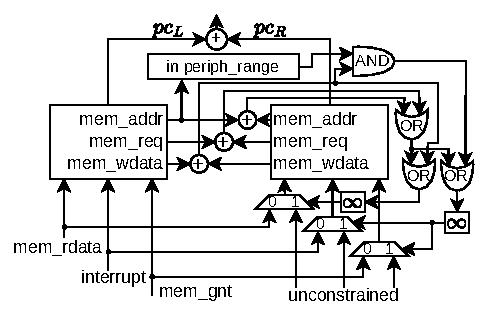
\includegraphics[width=0.9\columnwidth]{figures/picinstrum_miter/picinstrum_miter.pdf}
    \end{center}
    \vspace*{-1em}
    \caption{\Pici for a design whose information flows are tracked with a miter. }
    \label{fig:pic_instrum_miter}
    \vspace*{-.4em}
\end{figure}



% \section{Introduction}
% This document is a model and instructions for \LaTeX.
% Please observe the conference page limits.

% \section{Ease of Use}

% \subsection{Maintaining the Integrity of the Specifications}

% The IEEEtran class file is used to format your paper and style the text. All margins, 
% column widths, line spaces, and text fonts are prescribed; please do not 
% alter them. You may note peculiarities. For example, the head margin
% measures proportionately more than is customary. This measurement 
% and others are deliberate, using specifications that anticipate your paper 
% as one part of the entire proceedings, and not as an independent document. 
% Please do not revise any of the current designations.

% \section{Prepare Your Paper Before Styling}
% Before you begin to format your paper, first write and save the content as a 
% separate text file. Complete all content and organizational editing before 
% formatting. Please note sections \ref{AA}--\ref{SCM} below for more information on 
% proofreading, spelling and grammar.

% Keep your text and graphic files separate until after the text has been 
% formatted and styled. Do not number text heads---{\LaTeX} will do that 
% for you.

% \subsection{Abbreviations and Acronyms}\label{AA}
% Define abbreviations and acronyms the first time they are used in the text, 
% even after they have been defined in the abstract. Abbreviations such as 
% IEEE, SI, MKS, CGS, ac, dc, and rms do not have to be defined. Do not use 
% abbreviations in the title or heads unless they are unavoidable.

% \subsection{Units}
% \begin{itemize}
% \item Use either SI (MKS) or CGS as primary units. (SI units are encouraged.) English units may be used as secondary units (in parentheses). An exception would be the use of English units as identifiers in trade, such as ``3.5-inch disk drive''.
% \item Avoid combining SI and CGS units, such as current in amperes and magnetic field in oersteds. This often leads to confusion because equations do not balance dimensionally. If you must use mixed units, clearly state the units for each quantity that you use in an equation.
% \item Do not mix complete spellings and abbreviations of units: ``Wb/m\textsuperscript{2}'' or ``webers per square meter'', not ``webers/m\textsuperscript{2}''. Spell out units when they appear in text: ``. . . a few henries'', not ``. . . a few H''.
% \item Use a zero before decimal points: ``0.25'', not ``.25''. Use ``cm\textsuperscript{3}'', not ``cc''.)
% \end{itemize}

% \subsection{Equations}
% Number equations consecutively. To make your 
% equations more compact, you may use the solidus (~/~), the exp function, or 
% appropriate exponents. Italicize Roman symbols for quantities and variables, 
% but not Greek symbols. Use a long dash rather than a hyphen for a minus 
% sign. Punctuate equations with commas or periods when they are part of a 
% sentence, as in:
% \begin{equation}
% a+b=\gamma\label{eq}
% \end{equation}

% Be sure that the 
% symbols in your equation have been defined before or immediately following 
% the equation. Use ``\eqref{eq}'', not ``Eq.~\eqref{eq}'' or ``equation \eqref{eq}'', except at 
% the beginning of a sentence: ``Equation \eqref{eq} is . . .''

% \subsection{\LaTeX-Specific Advice}

% Please use ``soft'' (e.g., \verb|\eqref{Eq}|) cross references instead
% of ``hard'' references (e.g., \verb|(1)|). That will make it possible
% to combine sections, add equations, or change the order of figures or
% citations without having to go through the file line by line.

% Please don't use the \verb|{eqnarray}| equation environment. Use
% \verb|{align}| or \verb|{IEEEeqnarray}| instead. The \verb|{eqnarray}|
% environment leaves unsightly spaces around relation symbols.

% Please note that the \verb|{subequations}| environment in {\LaTeX}
% will increment the main equation counter even when there are no
% equation numbers displayed. If you forget that, you might write an
% article in which the equation numbers skip from (17) to (20), causing
% the copy editors to wonder if you've discovered a new method of
% counting.

% {\BibTeX} does not work by magic. It doesn't get the bibliographic
% data from thin air but from .bib files. If you use {\BibTeX} to produce a
% bibliography you must send the .bib files. 

% {\LaTeX} can't read your mind. If you assign the same label to a
% subsubsection and a table, you might find that Table I has been cross
% referenced as Table IV-B3. 

% {\LaTeX} does not have precognitive abilities. If you put a
% \verb|\label| command before the command that updates the counter it's
% supposed to be using, the label will pick up the last counter to be
% cross referenced instead. In particular, a \verb|\label| command
% should not go before the caption of a figure or a table.

% Do not use \verb|\nonumber| inside the \verb|{array}| environment. It
% will not stop equation numbers inside \verb|{array}| (there won't be
% any anyway) and it might stop a wanted equation number in the
% surrounding equation.

% \subsection{Some Common Mistakes}\label{SCM}
% \begin{itemize}
% \item The word ``data'' is plural, not singular.
% \item The subscript for the permeability of vacuum $\mu_{0}$, and other common scientific constants, is zero with subscript formatting, not a lowercase letter ``o''.
% \item In American English, commas, semicolons, periods, question and exclamation marks are located within quotation marks only when a complete thought or name is cited, such as a title or full quotation. When quotation marks are used, instead of a bold or italic typeface, to highlight a word or phrase, punctuation should appear outside of the quotation marks. A parenthetical phrase or statement at the end of a sentence is punctuated outside of the closing parenthesis (like this). (A parenthetical sentence is punctuated within the parentheses.)
% \item A graph within a graph is an ``inset'', not an ``insert''. The word alternatively is preferred to the word ``alternately'' (unless you really mean something that alternates).
% \item Do not use the word ``essentially'' to mean ``approximately'' or ``effectively''.
% \item In your paper title, if the words ``that uses'' can accurately replace the word ``using'', capitalize the ``u''; if not, keep using lower-cased.
% \item Be aware of the different meanings of the homophones ``affect'' and ``effect'', ``complement'' and ``compliment'', ``discreet'' and ``discrete'', ``principal'' and ``principle''.
% \item Do not confuse ``imply'' and ``infer''.
% \item The prefix ``non'' is not a word; it should be joined to the word it modifies, usually without a hyphen.
% \item There is no period after the ``et'' in the Latin abbreviation ``et al.''.
% \item The abbreviation ``i.e.'' means ``that is'', and the abbreviation ``e.g.'' means ``for example''.
% \end{itemize}
% An excellent style manual for science writers is \cite{b7}.

% \subsection{Authors and Affiliations}
% \textbf{The class file is designed for, but not limited to, six authors.} A 
% minimum of one author is required for all conference articles. Author names 
% should be listed starting from left to right and then moving down to the 
% next line. This is the author sequence that will be used in future citations 
% and by indexing services. Names should not be listed in columns nor group by 
% affiliation. Please keep your affiliations as succinct as possible (for 
% example, do not differentiate among departments of the same organization).

% \subsection{Identify the Headings}
% Headings, or heads, are organizational devices that guide the reader through 
% your paper. There are two types: component heads and text heads.

% Component heads identify the different components of your paper and are not 
% topically subordinate to each other. Examples include Acknowledgments and 
% References and, for these, the correct style to use is ``Heading 5''. Use 
% ``figure caption'' for your Figure captions, and ``table head'' for your 
% table title. Run-in heads, such as ``Abstract'', will require you to apply a 
% style (in this case, italic) in addition to the style provided by the drop 
% down menu to differentiate the head from the text.

% Text heads organize the topics on a relational, hierarchical basis. For 
% example, the paper title is the primary text head because all subsequent 
% material relates and elaborates on this one topic. If there are two or more 
% sub-topics, the next level head (uppercase Roman numerals) should be used 
% and, conversely, if there are not at least two sub-topics, then no subheads 
% should be introduced.

% \subsection{Figures and Tables}
% \paragraph{Positioning Figures and Tables} Place figures and tables at the top and 
% bottom of columns. Avoid placing them in the middle of columns. Large 
% figures and tables may span across both columns. Figure captions should be 
% below the figures; table heads should appear above the tables. Insert 
% figures and tables after they are cited in the text. Use the abbreviation 
% ``Fig.~\ref{fig}'', even at the beginning of a sentence.

% \begin{table}[htbp]
% \caption{Table Type Styles}
% \begin{center}
% \begin{tabular}{|c|c|c|c|}
% \hline
% \textbf{Table}&\multicolumn{3}{|c|}{\textbf{Table Column Head}} \\
% \cline{2-4} 
% \textbf{Head} & \textbf{\textit{Table column subhead}}& \textbf{\textit{Subhead}}& \textbf{\textit{Subhead}} \\
% \hline
% copy& More table copy$^{\mathrm{a}}$& &  \\
% \hline
% \multicolumn{4}{l}{$^{\mathrm{a}}$Sample of a Table footnote.}
% \end{tabular}
% \label{tab1}
% \end{center}
% \end{table}

% \begin{figure}[htbp]
% \centerline{
\includegraphics{fig1.png}}
% \caption{Example of a figure caption.}
% \label{fig}
% \end{figure}

% Figure Labels: Use 8 point Times New Roman for Figure labels. Use words 
% rather than symbols or abbreviations when writing Figure axis labels to 
% avoid confusing the reader. As an example, write the quantity 
% ``Magnetization'', or ``Magnetization, M'', not just ``M''. If including 
% units in the label, present them within parentheses. Do not label axes only 
% with units. In the example, write ``Magnetization (A/m)'' or ``Magnetization 
% \{A[m(1)]\}'', not just ``A/m''. Do not label axes with a ratio of 
% quantities and units. For example, write ``Temperature (K)'', not 
% ``Temperature/K''.

% \section*{Acknowledgment}

% The preferred spelling of the word ``acknowledgment'' in America is without 
% an ``e'' after the ``g''. Avoid the stilted expression ``one of us (R. B. 
% G.) thanks $\ldots$''. Instead, try ``R. B. G. thanks$\ldots$''. Put sponsor 
% acknowledgments in the unnumbered footnote on the first page.

% \section*{References}

% Please number citations consecutively within brackets \cite{b1}. The 
% sentence punctuation follows the bracket \cite{b2}. Refer simply to the reference 
% number, as in \cite{b3}---do not use ``Ref. \cite{b3}'' or ``reference \cite{b3}'' except at 
% the beginning of a sentence: ``Reference \cite{b3} was the first $\ldots$''

% Number footnotes separately in superscripts. Place the actual footnote at 
% the bottom of the column in which it was cited. Do not put footnotes in the 
% abstract or reference list. Use letters for table footnotes.

% Unless there are six authors or more give all authors' names; do not use 
% ``et al.''. Papers that have not been published, even if they have been 
% submitted for publication, should be cited as ``unpublished'' \cite{b4}. Papers 
% that have been accepted for publication should be cited as ``in press'' \cite{b5}. 
% Capitalize only the first word in a paper title, except for proper nouns and 
% element symbols.

% For papers published in translation journals, please give the English 
% citation first, followed by the original foreign-language citation \cite{b6}.

\bibliographystyle{IEEEtran}
\bibliography{main.bib}

\end{document}
